% FILENAME: paper/paper.tex

\documentclass[aps,prd,onecolumn,nofootinbib,11pt]{revtex4-2}

% FILENAME: paper/preamble.tex

% This file contains all the macros, packages, and setup for LuaLaTeX.

\usepackage{amsmath,amssymb}
\usepackage{graphicx}
\usepackage{hyperref}
\usepackage{minted}
\usepackage{xcolor}
\usepackage{xspace}
\usepackage{fontspec}
\usepackage{float}   % Added for [H] listing placement
\usepackage{slashed} % Added for Dirac \slashed{D} notation
\setmonofont{DejaVu Sans Mono}[Scale=MatchLowercase]

% --- Custom Macros ---
\newcommand{\todo}[1]{{\color{red}\bfseries [TODO: #1]}}
\newcommand{\spinFourC}{\ensuremath{\mathrm{Spin}(4, \mathbb{C})}\xspace}
\newcommand{\suTwo}{\ensuremath{\mathrm{Su}(2)}\xspace}
\newcommand{\slTwoC}{\ensuremath{\mathrm{SL}(2, \mathbb{C})}\xspace}
\newcommand{\slTwoCL}{\ensuremath{\mathrm{SL}(2, \mathbb{C})_L}\xspace}
\newcommand{\slTwoCR}{\ensuremath{\mathrm{SL}(2, \mathbb{C})_R}\xspace}
\newcommand{\slTwoCAlgL}{\ensuremath{\mathfrak{sl}(2, \mathbb{C})_L}\xspace}
\newcommand{\slTwoCAlgR}{\ensuremath{\mathfrak{sl}(2, \mathbb{C})_R}\xspace}

% --- Minted Setup ---
\setminted{
    linenos,
    breaklines,
    frame=lines,
    framesep=2mm,
    fontsize=\footnotesize,
    bgcolor=gray!5
}

% --- Lean Theorem Citation System ---
\newcounter{leancnt}
\newwrite\leanfile

% Open the auxiliary file for writing at the start of the document
% We immediately write \relax so the file is never mathematically 0 bytes.
\AtBeginDocument{%
    \immediate\openout\leanfile=\jobname.leanrefs
    \immediate\write\leanfile{\string\relax}
}

\makeatletter
% Command to use inside/outside equations: \leanref{TheoremName}
\newcommand{\leanref}[1]{%
    \ifmeasuring@
        % amsmath pass 1 (measuring): Output dummy width, don't increment or write.
        \ifmmode {}^{\textnormal{[L?]}} \else \textsuperscript{[L?]} \fi
    \else
        % pass 2 (rendering) or normal text mode:
        % Check if we have already assigned an ID to this specific theorem.
        \expandafter\ifx\csname lean@ref@id@\detokenize{#1}\endcsname\relax
            % FIRST TIME SEEN: Increment counter and assign ID globally (\xdef).
            \refstepcounter{leancnt}%
            \expandafter\xdef\csname lean@ref@id@\detokenize{#1}\endcsname{\theleancnt}%
            % Write the new entry to the index file.
            \immediate\write\leanfile{%
                \string\noindent\string\textbf{[L\theleancnt]}\string\quad%
                \string\texttt{\string\detokenize{#1}}\string\par\string\vspace{0.5em}%
            }%
        \fi
        % Output the superscript marker (either in math mode or text mode).
        \ifmmode 
            {}^{\textnormal{[L\csname lean@ref@id@\detokenize{#1}\endcsname]}}%
        \else 
            \textsuperscript{[L\csname lean@ref@id@\detokenize{#1}\endcsname]}%
        \fi
    \fi
}
\makeatother

% Command to drop the table of theorems at the end of the paper
\newcommand{\printleanrefs}{%
    \section*{Formal Verification Index}%
    \noindent The equations annotated with \textbf{[L$n$]} in the main text have been formally verified. They correspond to the following theorem signatures in the Lean 4 codebase:
    \par\vspace{1em}
    \immediate\closeout\leanfile
    \input{\jobname.leanrefs}
}


\begin{document}

\title{Chiral Gauge Dynamics: Formally Verified Emergence of Gravity, Quantum Mechanics, and Topological Matter from a \spinFourC Connection}
\author{Logan P. Evans}
\email{evanslp@uw.edu}
\affiliation{University of Washington}
\date{\today}

\begin{abstract}
Abstract
\end{abstract}

\maketitle

% --- INCLUDED SECTIONS ---
% FILENAME: paper/section-Introduction.tex

\section{Introduction}
\label{sec:Introduction}

In this paper, we explore an ontological foundation for the Einstein Field Equations (EFE). We extend the pure gauge connection formulation for gravity by showing that General Relativity emerges from a \spinFourC pure gauge connection. However, whereas the previously known \suTwo pure gauge formulation contains General Relativity, it does not natively contain particles. In contrast, a universe composed of only a \spinFourC connection contains General Relativity \textit{and} particles.

This research extensively uses the lean 4 mathematical formalization language \cite{deMoura2015lean}. The reason for this is simple: when we first discovered the mathematical structures that emerge from \spinFourC, which touch on problems related to quantum gravity, entanglement, measurement, dark energy, dark matter, and the origin of time, we were certain we had made a mathematical error. By formalizing the derivations in lean 4, we have eliminated the possibility that the math is incorrect. It's still possible that the theorems we prove here have no association with real physical phenomena, and lean 4 makes absolutely no claims about whether the \spinFourC gauge connection is ontologically correct for our universe. Also, due to the nascent state of the lean 4 ecosystem, our use of peer-reviewed literature exposes another possible avenue for errors.

In an ideal world, all of the physics literature we rely upon would be fully formalized from basic mathematical axioms, but that does not exist, so we created the Litlib library of transcriptions from published literature into lean 4 code. The lean 4 environment treats these transcriptions as axiomatically true, so we have to first trust that the papers were in fact correct, and then we have scrape up even more trust that the transcriptions into lean 4 are accurate.

We refer to this research program as Chiral Gauge Dynamics (CGD) because much of the rich mathematical structure comes from the chiral split $\spinFourC \cong \slTwoCL \times \slTwoCR$. Gauge theory, and in particular Yang-Mills theory \cite{yang1954conservation}, describes how elements of a field relate to each other regardless of the choice of coordinates. Since its introduction, it has undisputedly become the language of the Standard Model.

However, it wasn't until \citet{plebanski1977separation} that physicists knew that General Relativity could also be written as a gauge theory \citep{krasnov2011plebanski}. While this self-dual 2-forms formulation is not how General Relativity is taught in undergraduate classrooms, it is of vital importance to CGD.

Then \citet{ashtekar1986new} introduced \citeauthor{ashtekar1986new} variables, which showed that the gauge connection itself could produce General Relativity. With this result, General Relativity looked exactly like a Yang-Mills theory. It is interesting to note that this is the point in history where the research path that led to CGD diverged from the path that led to Loop Quantum Gravity (LQG) \citep{rovelli2008loop}. While the mathematical results of LQG and CGD are vastly different, at this historical fork in the road, the difference is that LQG quantized spacetime while CGD leaves spacetime as a classical field.

The mathematical insight that makes CGD possible is the astonishingly elegant Urbantke metric presented in \cite{urbantke1984integrability}. This work shows that a metric necessarily emerges for \suTwo and \spinFourC gauge fields. Intuitively, this describes the distance between two points by measuring the amount of twist in the field between two points.

The work first introduced in \citet{capovilla1989general} and later expanded in \citet{capovilla1991pure} took the Urbantke metric and showed that for a \suTwo pure gauge connection, General Relativity emerges without depending on a separate axiom for a background metric. We extend this result by showing that General Relativity also emerges from a \spinFourC pure gauge connection. However, while a universe composed only of a \suTwo connection contains General Relativity, it does not natively contain particles. In contrast, a universe composed of only a \spinFourC connection contains General Relativity as well as particles.

In Section \ref{sec:Foundations}, we will lay out the three CGD axioms:

\begin{itemize}
    \item Axiom 1: The universe is a classical \spinFourC gauge connection.
    \item Axiom 2: Macroscopic volume exists. This is a mathematical necessity for the lean 4 formalization to ignore trivial solutions. Conceptually it says, "There universe contains \textit{something} rather than \textit{nothing}."
    \item Axiom 3: The vacuum is unimodular. Tensor transformations, such as stretching, twisting, and compression, do not change the volume of spacetime.
\end{itemize}

\noindent In this section, we will also derive the Lagrangian and the Bianchi identities that govern stress-energy conservation and motion.

In Section \ref{sec:Gravity} we will prove that \spinFourC gives rise to General Relativity. This derivation takes us through the CDJ constraints \citep{capovilla1991pure}, Ricci-flat emergent spacetime, and stress-energy conservation.

Once we have formalized the existence of gravity within CGD, we will shift our focus in Section \ref{sec:matter} and show how the curvature of the \slTwoCR chiral sector acts as a physical matter source term. Skyrmion particles \citep{skyrme1962unified} emerge from CGD as topological defects where the metric becomes degenerate but where stable knots form. We will demonstrate confinement and three colors for these particles. Furthermore, we will show how a topological mass gap must exist for these particles.

Perhaps the most surprising aspect of CGD comes in Section \ref{sec:Quantum}, where we will derive the Dirac equation and the Born rule. We also derive entanglement and demonstrate that correlations of entangled particles match the Tsirelson bound. While this seems at first glance like a contradiction because CGD is a classical field theory, CGD entanglement bypasses Bell's theorem by challenging the assumption that two entangled particles are separate.

Finally, at the end of this paper in Section \ref{sec:ProtonRadius}, we will turn our focus on phenomenology. Most of the theoretical work presented in this paper focuses on showing how various physical theories emerge from \spinFourC. In a few places, our derivations require some nuance that is different between CGD and the Standard Model. However, in once case, CGD requires a feature that is starkly different: it requires the presence of an isovector axial-vector condensate. If such a condensate exists, it should have a substantial impact on the proton radius puzzle. When we first identified this, we assumed it would be an easy way to falsify the CGD theory. However, we created a one-parameter mathematical model that not only substantially outperformed the leading Standard Model empirical model, it also correctly identified the proton radius. We cannot argue that CGD solves the proton radius puzzle, but our assumption that this would be a quick and easy falsification turned out to be wrong.

In the appendices, we briefly summarize other proofs found within the lean 4 code. This includes several observations about cosmology.

\todo{Author (Final Polish): Update this appendix summary sentence once the paper is complete. Ensure it mentions:
\begin{itemize}
    \item Appendix A: Formal Verification Methodology and Litlib.
    \item Appendix B: Lean 4 Code Summary (The theorem signatures).
    \item Appendix C (or wherever it lands): Global Symmetries and Cosmological Boundary Conditions (The Big Bang / Hartle-Hawking Euclidean bounce proofs).
\end{itemize}}


% FILENAME: paper/section-Foundations.tex

\section{Foundations: The Topological Engine}
\label{sec:Foundations}

\subsection{The Core Ontology}
\label{subsec:core_ontology}

The core axiom of CGD is that the universe is a \spinFourC gauge connection. That's it. The \spinFourC field is a 4-dimensional space that acts like Jello where you can grab a clump, spin it around, and after you spin it through two complete rotations, it comes back to the original state without ever ripping any of the Jello.

However, \spinFourC is consistent with the trivial solution where there is no universe, so we need a second axiom to assert that the universe does, in fact, exist. To bridge this gap, we require a second axiom: the universe has non-trivial volume.

Of particular note are the axioms that are missing from CGD. \spinFourC has no independent background metric (required by standard General Relativity) and it has no fundamental quantization (required by the Standard Model and Loop Quantum Gravity \citep{ashtekar1986new}). We do not assert that time exists, that spacetime is Lorentz invariant, the Principle of Least Action, or that particles such as electrons and photons exist.

To formally represent the CGD axioms, we take the set of arbitrary 4-dimensional fields $\mathcal{A}_\mu(x) \in M_4(\mathbb{C})$ and constrain it to only the \spinFourC subset.

\begin{align}
    &\mathcal{A}_\mu(x) = A^{(L)}_\mu(x) \oplus A^{(R)}_\mu(x) \equiv
    \begin{pmatrix}
        A^{(L)}_\mu(x) & \begin{matrix} 0 & 0 \\ 0 & 0 \end{matrix} \\
        \begin{matrix} 0 & 0 \\ 0 & 0 \end{matrix} & A^{(R)}_\mu(x)
    \end{pmatrix}_{4 \times 4}, \nonumber \\
    \text{with} \quad &\text{Tr} \left( A^{(L)}_\mu \right) = \text{Tr} \left( A^{(R)}_\mu \right) = 0.
    \label{eq:chiral_split}
\end{align}

We represent the self-dual chiral sector as $A^{(L)}$ and the anti-self-dual chiral sector as $A^{(R)}$. Since the \spinFourC algebra decomposes into the sum of the self-dual and anti-self-dual chiral algebras $\slTwoCAlgL \oplus \slTwoCAlgR$, we embed them as block-diagonal components of a 4-dimensional matrix. In order to disable scaling operations, the trace of $A_\mu(x)$ must equal zero; the only operations allowed are boosts (accelerations in a direction) and spins (a rotation around an axis). Finally, since CGD is a classical theory, the \spinFourC field must be differentiable everywhere, represented by requiring $A^{(L)}_\mu, A^{(R)}_\mu \in C^\infty(\mathbb{R}^4)$.

Within the Lean 4 formalization, we encode \spinFourC by writing

\begin{listing}[H]
\begin{minted}{lean}
-- CGD.Axioms.Ontology
structure Universe where
  val : Fin 4 → SpacetimePoint → ChiralM

  is_spin4c : ∀ mu x, val mu x = 
    embedSelfDual (chiralProject (val mu x)).self_dual + 
    embedAntiSelfDual (chiralProject (val mu x)).anti_self_dual

  sd_is_smooth : ∀ mu i j, ContDiff ℝ ⊤
    (fun x => (chiralProject (val mu x)).self_dual.val i j)
  asd_is_smooth : ∀ mu i j, ContDiff ℝ ⊤
    (fun x => (chiralProject (val mu x)).anti_self_dual.val i j)
\end{minted}
\caption{The foundational definition of the universe as a continuous \spinFourC gauge field.}
\label{lean:Universe}
\end{listing}

and we encode the existence of the universe by writing

\begin{listing}[H]
\begin{minted}{lean}
-- CGD.Axioms.Phenomenology
class MacroscopicVolume (u : Universe) (bulk : Set SpacetimePoint) : Prop where
  volume_exists : ∀ x ∈ bulk, (urbantkeMetric (fun μ ν => curvatureSl2c u.sd_sector μ ν x)).det ≠ 0
\end{minted}
\caption{The phenomenological volume axiom requiring non-degenerate geometry.}
\label{lean:MacroscopicVolume}
\end{listing}

The \spinFourC gauge connection is not arbitrary. Instead, it satisfies several properties required to make the universe work. In order to represent time and to represent Dirac spinors (Section \ref{subsec:emergent_dirac}), we require a 4-dimensional space. Since CGD does not postulate a distance metric, we will need to use the Urbantke metric (Section \ref{subsec:unimodular_cdj}) to obtain one. However, the Urbantke metric only works for \suTwo or \spinFourC \citep{urbantke1984integrability}, and \suTwo is eliminated because it is 3-dimensional.

As soon as we select the \spinFourC gauge connection, an astonishing mathematical property emerges: \spinFourC is isomorphic to $\slTwoCL \oplus \slTwoCR$. This is the only complexified gauge group that decomposes into two orthogonal chiral halves. Returning to the Jello metaphor, this means that if you take a clump of Jello and throw it like a football with a perfect spiral, then the footballs thrown by a left-handed and a right-handed quarterback will pass through each other without interfering. While this algebraic independence is a type of superposition, it is not quantum superposition, and in fact, we will see in Section \ref{sec:Quantum} that quantum mechanics in CGD doesn't use superposition at all. Instead, we will show in Section \ref{subsec:schroedinger_limit} that superposition is important to generate mass.

\subsection{The Absence of a Dynamical Lagrangian}
\label{subsec:absence_of_lagrangian}

We represent the geometric constraints of CGD using the Lagrangian

\begin{align}
    \mathcal{L}_{\text{CGD}} 
    &= \text{Tr}(F \wedge F) \nonumber \\
    &= -\frac{1}{2} \sum_{\mu,\nu,\rho,\sigma} \epsilon^{\mu\nu\rho\sigma} \text{Tr}(F_{\mu\nu} F_{\rho\sigma}) \quad \leanref{CGD.Foundations.Lagrangian.topologicalLagrangianUniqueness} \nonumber \\
    &= \mathcal{L}_{\text{vac}}\left(F^{(L)}_{\mu\nu}\right) + \mathcal{L}_{\text{ASD}}\left(F^{(R)}_{\mu\nu}\right) \quad \leanref{CGD.Foundations.ChiralDecomposition.algebraicChiralDecomposition} .
    \label{eq:master_lagrangian}
\end{align}

\noindent While we have three equivalent ways to write the Lagrangian, $\mathcal{L} = \mathcal{L}_{\text{vac}}\left(F^{(L)}_{\mu\nu}\right) + \mathcal{L}_{\text{ASD}}\left(F^{(R)}_{\mu\nu}\right)$, where vac represents the self-dual vacuum and ASD represents the anti-self-dual sector, is the notation that emphasizes that the CGD universe is made up of two chiral halves.

In order to do physics in a universe with no independent background metric, we need to bootstrap a way to measure direction and distance. So far, the only thing we're able to measure in \spinFourC is topological twists. However, \citet{utiyama1956invariant} showed that gauge invariance forces the Lagrangian to be the trace of the curvature squared. Since no background metric exists, the unique Lagrangian that satisfies this constraint is $-\frac{1}{2} \sum_{\mu,\nu,\rho,\sigma} \epsilon^{\mu\nu\rho\sigma} \text{Tr}(F_{\mu\nu} F_{\rho\sigma})$ \citep{nakahara2003geometry}.

Typically, we could use the Lagrangian of a system to give us the action, and by varying the action we can find the equations of motion and extract a distance metric. However, with the Utiyama Lagrangian, when we build the action and then vary it, we get exactly zero.

\begin{align}
    S[A] &= \int \mathcal{L}(F_{\mu\nu}) \, d^4x \quad \leanref{CGD.Foundations.Action.universeAction} \nonumber \\
    \left. \frac{d}{d\tau} S[v(\tau)] \right|_{\tau=0} &= 0 \quad \leanref{CGD.Foundations.Lagrangian.topologicalActionVariationZero}
    \label{eq:topologicalActionVariationZero}
\end{align}

\noindent In other words, while we have a Lagrangian, we cannot use Euler-Lagrange equations to obtain a distance metric, the equation of state, or equations of motion.

Instead, we turn to a metric that natively lives within the \spinFourC topology \citep{urbantke1984integrability}. The Urbantke metric is the unique conformal metric that forces a \slTwoC gauge field to be self-dual. Specifically,

\begin{equation}
    g_{\mu\nu} = \sum_{a,b,c=1}^3 \sum_{\alpha,\beta,\gamma,\delta=0}^3 \epsilon_{abc} \epsilon^{\alpha\beta\gamma\delta} F^a_{\mu\alpha} F^b_{\nu\beta} F^c_{\gamma\delta}.
    \quad \leanref{CGD.Gravity.Geometry.urbantkeMetric}
    \label{eq:urbantke_metric}
\end{equation}

\noindent This metric exists independently for both the \slTwoCL and \slTwoCR chiral halves. At this point, we have a metric and a Lagrangian, but we do not yet know if the metric collapses or if particles exist. In the next section we will explore what happens to the metric in both chiral halves as we show how gravity and the equations of motion emerge from \spinFourC.


% FILENAME: paper/section-Gravity.tex

\section{Gravity: The Emergence of Spacetime}
\label{sec:Gravity}

\subsection{The Vacuum Condensate and Time Emergence}
\label{subsec:vacuum_condensate}

\todo{Author: Explain that space is not an empty stage; "empty" space mathematically has zero volume. State that a non-degenerate macroscopic metric ($\det(g) \neq 0$) requires a non-trivial gauge field condensate. Argue that a static universe also collapses to zero volume; thus, time evolution is geometrically required for space to exist.}

\begin{equation}
    \det(g_{\mu\nu}) \neq 0 \implies A^{(L)}_\mu \neq 0
    \label{eq:kinematicVacuumCondensate}
\end{equation}

\begin{listing}[H]
\begin{minted}{lean}
-- CGD.Quantum.Vacuum
theorem kinematicVacuumCondensate (u : Universe) (bulk : Set SpacetimePoint)
  [vol : CGD.Axioms.MacroscopicVolume u bulk] (x : SpacetimePoint) (hx : x ∈ bulk) :
  u.sd_sector.val ≠ (fun _ _ => 0)
\end{minted}
\caption{Proof that a non-zero spacetime volume forbids the trivial vacuum.}
\label{lean:kinematicVacuumCondensate}
\end{listing}

\begin{equation}
    \partial_0 A_i = 0 \implies \det(g_{\mu\nu}) = 0
    \label{eq:kinematicStaticUniverseDegeneracy}
\end{equation}

\begin{listing}[H]
\begin{minted}{lean}
-- CGD.Cosmology.BigBang
theorem kinematicStaticUniverseDegeneracy (u : Universe) :
  isStaticUniverse u →
  ∀ x, (urbantkeMetric (fun mu nu => curvatureSl2c u.sd_sector mu nu x)).det = 0
\end{minted}
\caption{A purely static universe collapses the emergent geometric volume to zero.}
\label{lean:kinematicStaticUniverseDegeneracy}
\end{listing}

\begin{equation}
    F_{\mu\nu} = \frac{1}{2} \epsilon_{\mu\nu}^{\phantom{\mu\nu}\rho\sigma} F_{\rho\sigma} \implies \text{Metric signature is degenerate or Euclidean}
    \label{eq:kinematicTimeEmergence}
\end{equation}

\begin{listing}[H]
\begin{minted}{lean}
-- CGD.Cosmology.TimeEmergence.Theorem
theorem kinematicTimeEmergence (u : Universe) (phaseRegion : Set SpacetimePoint)
  (h_symm : ∀ x ∈ phaseRegion, isFully4DSymmetric (fun mu nu => curvatureSl2c u.sd_sector mu nu x)) :
  ∀ x ∈ phaseRegion,
    ¬ isLorentzian (urbantkeMetric (fun m n => curvatureSl2c u.sd_sector m n x))
\end{minted}
\caption{A Lorentzian time axis is forbidden without spontaneous Euclidean symmetry breaking.}
\label{lean:kinematicTimeEmergence}
\end{listing}

\subsection{Unimodular CDJ Gravity}
\label{subsec:unimodular_cdj}

\todo{Author: Since we lack equations of motion, introduce the Capovilla-Dell-Jacobson (CDJ) algebraic constraint framework. Explain that the Cosmological Constant ($\Lambda$) is not manually inserted into an action, but emerges purely as an integration constant from the unimodular topological requirement.}

\begin{equation}
    \det(g_{\mu\nu}) = c \propto \Lambda^3 \neq 0
    \label{eq:macroscopicVacuumEmergence}
\end{equation}

\begin{listing}[H]
\begin{minted}{lean}
-- CGD.Gravity.DomainSeparation
theorem macroscopicVacuumEmergence 
  (u : Universe) (Λ : ℂ) (bulkVacuum : Set SpacetimePoint)
  (h_Λ_neq_zero : Λ ≠ 0) (k : ℂ) (hk : k ≠ 0)
  ... [Urbantke matrix adapter definition elided] ...
  (h_vacuum : isVacuumRegion bulkVacuum u Λ) :
  ∃ (c : ℂ), c ≠ 0 ∧ ∀ x y : bulkVacuum, 
    (cgdUnimodularMetricAdapter (fun m n => cgdAdjointCurvature u m n x.val)).det = c
\end{minted}
\caption{The Unimodular emergence of a constant macroscopic volume tied to $\Lambda$.}
\label{lean:macroscopicVacuumEmergence}
\end{listing}

\begin{equation}
    R_{\mu\nu} = 0
    \label{eq:macroscopicRicciFlatEmergence}
\end{equation}

\begin{listing}[H]
\begin{minted}{lean}
-- CGD.Gravity.DomainSeparation
theorem macroscopicRicciFlatEmergence
  (u : Universe) (urbantke_tetrad : TetradField)
  (metric_compat : ∀ x μ ν, metricFromTetrad urbantke_tetrad μ ν x = 
                           CGD.Gravity.urbantkeMetric (fun m n => curvatureSl2c u.sd_sector m n x) μ ν)
  ... [Capovilla-Dell-Jacobson constraints (Eq 2.2b/c) elided] ...
  (bulkVacuum : Set SpacetimePoint) (hOpen : IsOpen bulkVacuum) :
  ∀ x ∈ bulkVacuum, ∀ μ ν, ricciTensor (fun m n p => urbantkeMetric (fun a b => curvatureSl2c u.sd_sector a b p) m n) μ ν x = 0
\end{minted}
\caption{The derivation of Ricci-flat General Relativity via the Capovilla-Dell-Jacobson constraint.}
\label{lean:macroscopicRicciFlatEmergence}
\end{listing}

\subsection{Exact Lorentzian Macroscopic Witness}
\label{subsec:exact_lorentzian}

\todo{Author: Emphasize that this theorem is a \textbf{Capstone}. To prove this framework isn't just a vacuous Euclidean toy model, we have analytically verified an exact SU(2) gauge configuration that yields a strictly non-degenerate, negative determinant, Lorentzian spacetime metric at the origin.}

\begin{equation}
    \Sigma^{ab} - \frac{1}{3}\delta^{ab}\text{Tr}(\Sigma) = 0 \quad \text{and} \quad \det(g_{\mu\nu}) < 0
    \label{eq:dynamicExactLorentzianSolution}
\end{equation}

\begin{listing}[H]
\begin{minted}{lean}
-- CGD.Gravity.ExactSolutions.MainTheorem
theorem dynamicExactLorentzianSolution :
  ∃ (u : Universe) (x : SpacetimePoint), 
    (∑ μ ν ρ σ, epsilon4 μ ν ρ σ • (cgdAdjointCurvature u μ ν x * cgdAdjointCurvature u ρ σ x)) = 
    ((∑ μ ν ρ σ, epsilon4 μ ν ρ σ • (cgdAdjointCurvature u μ ν x * cgdAdjointCurvature u ρ σ x)).trace / 3) • 1 ∧
    isLorentzian (urbantkeMetric (fun m n => curvatureSl2c u.sd_sector m n x))
\end{minted}
\caption{Formal construction of an exact non-Abelian field yielding a macroscopic Lorentzian metric.}
\label{lean:dynamicExactLorentzianSolution}
\end{listing}

\subsection{Machian Motion of Topological Defects}
\label{subsec:machian_motion}

\todo{Author: Return to the physicist's critique: if the topological action's variation is zero, how do things move? Explain that the emergent Urbantke metric natively satisfies the Bianchi identities, satisfying the Geroch-Jang theorem premises. Conclude that defects are strictly forced to travel along timelike geodesics.}

\begin{equation}
    \nabla_\mu T^{\mu\nu} = 0 \implies x^\mu(\tau) \text{ is a timelike geodesic}
    \label{eq:machianTopologicalDefectMotion}
\end{equation}

\begin{listing}[H]
\begin{minted}{lean}
-- CGD.Gravity.GeodesicMotion
theorem machianTopologicalDefectMotion
  (isFutureDirectedTimelike : SpacetimePoint → (Fin 4 → ℝ) → Prop)
  (isTimelikeGeodesic : Set SpacetimePoint → Prop)
  (u : Universe)
  ... [Manifold smoothness, Contracted Bianchi, and Litlib.GerochJang axioms elided] ...
  (T_real : Fin 4 → Fin 4 → SpacetimePoint → ℝ) (γ : Set SpacetimePoint)
  (h_T_real_def : ∀ mu nu x, T_real mu nu x = (emergentStressEnergy (fun a b p => curvatureSl2c u.sd_sector a b p) mu nu x).re)
  (h_dominant_energy : ∀ x, (∃ mu nu, T_real mu nu x ≠ 0) → ∀ t t', 
    isFutureDirectedTimelike x t → isFutureDirectedTimelike x t' → ∑ a, ∑ b, T_real a b x * t a * t' b > 0)
  (h_localized : ∀ U : Set SpacetimePoint, IsOpen U → γ ⊆ U → closure {x | ∃ mu nu, T_real mu nu x ≠ 0} ⊆ U) :
  isTimelikeGeodesic γ
\end{minted}
\caption{The mathematical necessity of timelike geodesic motion derived from geometry.}
\label{lean:machianTopologicalDefectMotion}
\end{listing}

% FILENAME: paper/section-Matter.tex

\section{Matter: Topological Knots and the SU(3) Problem}

\subsection{The Necessity of Non-Abelian Fields}
% TODO for Author: Explain why a U(1) Abelian field (like pure electromagnetism) cannot create space on its own. The volume determinant natively collapses. The universe absolutely requires non-Abelian fields (color) to expand into a macroscopic geometry.

\begin{equation}
    [F_{\mu\nu}, F_{\rho\sigma}] = 0 \implies \det(g_{\mu\nu}) = 0
\end{equation}
\begin{minted}{lean}
-- CGD.Particles.Color
theorem kinematicSingleColorDegeneracy :
  ∀ (F : Fin 4 → Fin 4 → SL2C),
    isSingleColor F →
    (urbantkeMetric F).det = 0
\end{minted}

\subsection{Topological Stability}
% TODO for Author: Explain that particles are not point masses added to the universe; they are stable topological knots (instantons) in the gauge field. Introduce the Cartan-Maurer degree / Belavin bounds to explain why these knots cannot mathematically decay or unwrap into the trivial vacuum.

\begin{equation}
    \int_{S^3} \text{Cartan-Maurer Form} \neq 0 \implies A \text{ cannot decay to } 0
\end{equation}
\begin{minted}{lean}
-- CGD.Particles.TopologicalStability
theorem kinematicTopologicalStability 
  (windingNumber : (S3 → SU2Group) → ℤ)
  (cartanMaurerIntegral : (S3 → SU2Group) → ℝ)
  ... [Litlib.Belavin1975 and Nakahara Cartan-Maurer boundaries elided] ...
  (integral_zero : cartanMaurerIntegral 1 = 0) :
  ¬ isHomotopicConnection bpstInstanton 0
\end{minted}

\subsection{Geometric Confinement}
% TODO for Author: Address the "SU(3) Problem". Why don't we need a fundamental SU(3) gauge group for the Strong Force? Explain that multi-color components natively crush into 1D topological flux tubes (strings), perfectly yielding a 1D confining Hamiltonian.

\begin{equation}
    \mathcal{H}_{3D} \rightarrow \frac{1}{2} E_z^2 + \frac{1}{2} B^2 \quad \text{(1D Confinement Reduction)}
\end{equation}
\begin{minted}{lean}
-- CGD.Particles.Confinement
theorem kinematicStringConfinement :
  ∀ (E B : Matrix (Fin 3) (Fin 3) ℂ) (E_z : ℂ),
    isCrushedString E E_z →
    ∃ (v : Fin 3 → ℂ), (∑ i : Fin 3, v i * v i = 1) ∧
      densitizedHamiltonian E B = (1 / 2 : ℂ) * E_z^2 + (1 / 2 : ℂ) * ∑ a : Fin 3, ∑ b : Fin 3, B a b * B a b
\end{minted}

% FILENAME: paper/section-Quantum.tex

\todo{Author Overview: This section proves that standard quantum mechanical behavior—wave equations, quantization, and entanglement—emerges strictly from the geometric phase space of the topological connection.
Order of theorems covered:
1. generalizedDynamicDiracEquation / familiarDynamicDiracEquation
3. kinematicEntanglementWormhole / kinematicFluxTubeStability
4. relationalTimeEmergence
5. kinematicActionQuantization
6. fluxTubeHolonomyEvaluation / geometricHolonomyTsirelsonBound
8. finiteLiouvilleBoundaryFlow / kinematicBornRuleEquivalence
}

\section{Quantum Mechanics Without Quantization}
\label{sec:Quantum}

\subsection{The Emergent Dirac Operator}

\todo{Author: Because this is now the start of the section, change the transition word "Next" to something like "To begin our exploration into how quantum particles behave in CGD..." Also, regarding your mathcal question: yes, it is standard to use $\mathcal{A}$ for the connection to distinguish it from the $A$ electromagnetic vector potential. Just ensure it's consistent throughout the paper.}
Next, we will explore just how particles behave in CGD. As we discussed in Section \ref{Introduction}, \spinFourC naturally possesess a bispinor structure, so we will evaluate the Dirac operator $\slashed{D}$ by treating the local gauge connection as the spinor field $(\Psi = \mathcal{A}_\nu)$ \todo{did we miss the mathcal in other uses in other sections?}. By considering the gauge-covariant derivative and the Yang-Mills curvature tensor, we find
\begin{equation}
    D_\mu \mathcal{A}_\nu = F_{\mu\nu} + \partial_\nu \mathcal{A}_\mu .
    \quad \leanref{CGD.Quantum.covariantSpinorDeriv_eq_curvature_plus_deriv}
    \label{eq:covariantSpinorIdentity}
\end{equation}
\noindent When we contract this identity with the tetrad field $e_a^\mu$ and the Dirac gamma matrices $\gamma^a$, we obtain
\begin{equation}
    \slashed{D}_\nu \Psi = e_a^\mu \gamma^a F_{\mu\nu} + e_a^\mu \gamma^a (\partial_\nu \mathcal{A}_\mu)
    \quad \leanref{CGD.Quantum.generalizedDynamicDiracEquation}
    \label{eq:generalizedDynamicDiracEquation}
\end{equation}
\noindent This is the generalized Dirac Equation. In the first term, $F_{\mu\nu}$ is the interaction between a fermion and a gauge field. In the second term, $\partial_\nu \mathcal{A}_\mu$ is an intertial term. This means that particles feel a force from the background if the background universe is dynamically bubbling or expanding, but if the universe is stationary, the second term goes to zero and we recover the standard definition for the Dirac Equation.

\subsection{Entanglement and the ER=EPR Bridge}

Since CGD is a classical field theory for both gravity and particles, one of the biggest concerns is how it addresses Bell's Theorem. \citeauthor{bell1964einstein} concluded:
\begin{quote}
    In a theory in which parameters are added to quantum mechanics to determine the results of individual measurements, without changing the statistical predictions, there must be a mechanism whereby the set- ting of one measuring device can influence the reading of another instrument, however remote. Moreover, the signal involved must propagate instantaneously, so that such a theory could not be Lorentz invariant. \citep{bell1964einstein}
\end{quote}
\noindent This is colloquially summarized as ``No local, hidden-variables theory explains Quantum Mechanics.'' This is a problem for a theory like CGD because classical theories must be local hidden-variable theories in order to satisfy Lorentz Invariance.

However, \citet{maldacena2013cool} showed a loop-hole for Bell's Theorem when they introduced the ER=EPR hypothesis: if two particles are topologically inseparable, they can satisfy observed entanglement correlations without requiring any non-local behavior. While we will not use any part of the mechanism \citet{maldacena2013cool} discussed, we will show that the CGD math supports a 1-dimensional topological flux tube that connects entangled particles.

\todo{Author: Your sentence cuts off here. Finish the thought by formally introducing the `fluxTubeFrame` witness here. State that we evaluate the metric strictly inside this 1D core connecting two states, yielding a determinant of zero. This proves the geometric distance between the particles is zero, making them inseparable.}
In order to explore entanglement in CGD, we will start with the general quantum geometry we proved with CGD.Quantum.generalizedDynamicDiracEquation\leanref{CGD.Quantum.generalizedDynamicDiracEquation}, but in order to explore the possible behavior of the quantum geometry, we must use some 

\begin{equation}
    \det(g_{\mu\nu}) = 0 \quad \text{along the ER=EPR bridge}
    \quad \leanref{CGD.Quantum.kinematicEntanglementWormhole}
    \label{eq:kinematicEntanglementWormhole}
\end{equation}

\todo{Author: Explain how path-integrating the SU(2) holonomy along this flux tube purely recovers quantum state vectors and the macroscopic CHSH Tsirelson bound of $2\sqrt{2}$.}

\begin{equation}
    \left[ \text{Re}(\text{CHSH}) \right]^2 \leq 8
    \quad \leanref{CGD.Quantum.geometricHolonomyTsirelsonBound}
    \label{eq:geometricHolonomyTsirelsonBound}
\end{equation}
\todo{Cite Litlib Dependency: \cite{hall2000elementary} for the Lie derivative exponential maps required for macroscopic holonomy.}

\subsection{Relational Time}

\todo{Author: To answer your citation question: Cite Carlo Rovelli's "Relational Quantum Mechanics" (1996) or the Wheeler-DeWitt equation for the "problem of time".}
Since we proved in Equation \ref{eq:topologicalActionVariationZero} that CGD does not possess a classical Hamiltonian, the Dirac operator in Equation \ref{eq:generalizedDynamicDiracEquation} is not sufficient by itself to explain the complex phase rotation of quantum time-evolution. For this, we need to address ``the problem of time'' \todo{cite someone?}. 

\todo{Author: To answer your matrix exponential question: No, you do not need a times dot for $t \mathcal{A}$; standard juxtaposition is correct. Also, adjust the transition to the 1D core here by referencing the flux tube we just introduced in the previous subsection.}
First, we note that the path-integral of a connection $\mathcal{A}$ over distance $t$ is the matrix exponential of the field multiplied by the distance $(e^{t \mathcal{A}})$ \todo{do I need a times dot there?}. To evaluate this spatial holonomy, we must make a physical assumption that a defect possesses a 1-dimensional core 

 ... Also, we note that the quantum mechanical operator of an evolving system is $e^{-iHt}$.

\todo{Author: Bring this together. State that evaluating the spatial holonomy along the U(1) core of the flux tube mathematically mirrors $e^{-iHt}$, meaning time evolution is just relational geometric phase.}

\begin{equation}
    \mathcal{P} \exp \left( \int \mathcal{A}_1 dx^1 \right) = \exp(-i H t)
    \quad \leanref{CGD.Quantum.Holonomy.relationalTimeEmergence}
    \label{eq:relationalTimeEmergence}
\end{equation}

\subsection{Topological Quantization}

Canonical quantization is a mathematical process that turns a classical theory into a quantum theory. By treating classical quantities such as position or momentum as operators with the axiomatic non-commutation property $[\hat{q}, \hat{p}] = i \hbar$, physicists can obtain probability waves and discrete energy levels.

\todo{Author: To answer your group theory question: We use SU(2) instead of Spin(4,C) because Spin(4,C) is a "non-compact" group (it stretches to infinity). You cannot mathematically tie a stable knot in a non-compact group; it slips open. Stable topological defects can only form in compact subgroups, which is SU(2). To answer your theorem question: This is the Nakahara "Cartan-Maurer Degree Theorem".}
In CGD, we do not have the non-commutation property, so if quanta exist, they must emerge from the topology. However, since the background of the \spinFourC is a macroscopic \suTwo field, the \suTwo group manifold is a 3-dimensional sphere $S^3$. If we take a topological defect $(F^{(R)}_{\mu\nu} \neq 0)$, we can enclose it in another $S^3$ sphere at spatial infinity. At this boundary, we have a mathematical mapping $S^3 \to S^3$. To obtain quantization, we use \todo{what is the name of the theorem?} which shows that it is only possible to wrap a sphere with another sphere an integer number of times without tearing the manifold ($\pi_3(\suTwo) = \mathbb{Z}$) \todo{why not put \spinFourC in there instead of \suTwo?}. 

\todo{Author: To answer your question: The Cartan-Maurer integral is simply the calculus formula that computes the topological winding number over that $S^3$ boundary.}
Next, we consider the Pontryagin density that we proved is the unique CGD Lagrangian in Equation \ref{eq:topologicalLagrangianUniqueness}. Stokes' theorem proves that the volume integral of a derivative is equal to the value at its boundary, so when we integrate the 4-dimensional action, we find that that action possessed by the particle is quantized. Thus, the Cartan-Maurer integral \todo{what is that?} evaluates to
\begin{equation}
    S_{\text{top}} \in \{ -1, 1 \} .
    \quad \leanref{CGD.Quantum.kinematicActionQuantization}
    \label{eq:kinematicActionQuantization}
\end{equation}
\todo{Cite Litlib Dependency: \cite{belavin1975pseudoparticle} and \cite{nakahara2003geometry} for the topological degree mapping constraints.}

In CGD, the ``quantum'' is the geometric winding number for a topological defect.

\subsection{The Born Rule and Measurement}
\label{subsec:measurement}

\todo{Author: Conclude with the Born Rule. Explain that continuous gauge flow inherently preserves phase space volume (Liouville's theorem), and projecting this invariant volume exactly derives the $1 - M/E_0$ Born Rule probability.}

\begin{equation}
    P = \frac{\int_{\theta}^{\pi} d\mathcal{V}_{\text{Hopf}}}{\int_{0}^{\pi} d\mathcal{V}_{\text{Hopf}}} = 1 - \frac{M}{E_0}
    \quad \leanref{CGD.Quantum.Measurement.kinematicBornRuleEquivalence}
    \label{eq:kinematicBornRuleEquivalence}
\end{equation}
\todo{Cite Litlib Dependency: \cite{arnold1989mathematical} for the n-dimensional Liouville volume-preservation theorem.}

% FILENAME: paper/section-Cosmology.tex

\section{Cosmological Bounds and Compatibility Limits}
% TODO for Author: Provide a brief introductory paragraph stating that this section verifies the framework's compatibility with established physical limits (non-relativistic mechanics, cosmology, and asymptotic limits) without needing to rely on ad-hoc parameters.

\subsection{The Schrödinger Non-Relativistic Limit}
% TODO for Author: Explain that as a compatibility check, splitting the large and small components of the covariant Dirac field natively recovers the standard 1/2m non-relativistic Schrödinger Hamiltonian.

\begin{equation}
    2m \Psi_{\text{small}} = P_+ (\partial_0 \Psi + m \Psi) + \gamma^i P_- (\partial_i \Psi)
\end{equation}
\begin{minted}{lean}
-- CGD.Quantum.Schroedinger
theorem exactSchroedingerReduction (dPsi : Fin 4 → SpacetimePoint → Matrix (Fin 4) (Fin 4) Complex) 
  (Psi : SpacetimePoint → Matrix (Fin 4) (Fin 4) Complex) (m : Complex) (x : SpacetimePoint) :
  localDiracOp (fun a => dPsi a x) = m • Psi x →
  let D0_mod := modulatedTemporalDeriv (dPsi 0 x) (Psi x) m;
  let Psi_small := P_plus * Psi x;
  (2 • m • Psi_small = P_plus * D0_mod + gammaVec 1 * (P_minus * dPsi 1 x) + gammaVec 2 * (P_minus * dPsi 2 x) + gammaVec 3 * (P_minus * dPsi 3 x)) ∧
  (P_minus * D0_mod = gammaVec 1 * (P_plus * dPsi 1 x) + gammaVec 2 * (P_plus * dPsi 2 x) + gammaVec 3 * (P_plus * dPsi 3 x))
\end{minted}

\subsection{Non-Singular Cosmological Origins}
% TODO for Author: Explain how enforcing a topological boundary condition means the Big Bang manifests as a pure Euclidean SO(4) instanton bounce rather than a mathematical singularity. Additionally, explain how parity inversion naturally flips the topological charge, linking the arrow of time to matter/antimatter asymmetry.

\begin{equation}
    g_{\mu\nu} = c \delta_{\mu\nu}
\end{equation}
\begin{minted}{lean}
-- CGD.Cosmology.BigBang
theorem kinematicBigBang (u : Universe) (phaseRegion : Set SpacetimePoint)
  [vol : CGD.Axioms.MacroscopicVolume u phaseRegion]
  (h_symm : ∀ x ∈ phaseRegion, isFully4DSymmetric (fun mu nu => curvatureSl2c u.sd_sector mu nu x)) :
  ∀ x ∈ phaseRegion, ∃ c : Complex, c ≠ 0 ∧ urbantkeMetric (fun mu nu => curvatureSl2c u.sd_sector mu nu x) = c • 1
\end{minted}

\begin{equation}
    F_{0i} \to -F_{0i} \implies Q \to -Q
\end{equation}
\begin{minted}{lean}
-- CGD.Cosmology.ParityInversion
theorem kinematicParityInversion (u : Universe) :
  ∀ (x : SpacetimePoint) (P_F : Fin 4 → Fin 4 → SL2C),
    isParityInvertedTensor (fun m n => curvatureSl2c u.sd_sector m n x) P_F x →
    pontryaginDensity P_F = - pontryaginDensity (fun mu nu => curvatureSl2c u.sd_sector mu nu x)
\end{minted}

\subsection{Asymptotic String Breaking}
% TODO for Author: Briefly mention that while the 1D flux tube represents a confining Strong Force potential, topological crossover limits dictate that the string will eventually mathematically "snap" at macroscopic distances. 

\begin{equation}
    L > \frac{2M}{\sigma} \implies \text{String Breaking}
\end{equation}
\begin{minted}{lean}
-- CGD.Quantum.Entanglement.Decay
theorem algebraicStringBreakingLimit
  (energyFunc : (Fin 4 → SpacetimePoint → SL2C) → ℝ)
  (intactState snappedState : ℝ → Fin 4 → SpacetimePoint → SL2C)
  {sigma M : ℝ} [eb : FluxTubeStringBreaking (Fin 4 → SpacetimePoint → SL2C) energyFunc intactState snappedState sigma M]
  (u : Universe) (L : ℝ)
  (h_L_pos : L > 0)
  (h_intact : u.sd_sector = intactState L)
  (h_L_crossover : L > (2 * M) / sigma) :
  ¬ isGlobalMinimum energyFunc u.sd_sector
\end{minted}

% FILENAME: paper/section-Conclusion.tex

\todo{Author Overview: The victory lap. Summarize that we didn't add anything; we took a pure gauge connection and derived gravity, matter, and QM simply by applying strict geometry.}

\todo{Author: Review and rename section title if desired.}
\section{Conclusion and Future Outlook}
\label{sec:Conclusion}

\todo{Author: Recap the core thesis. We started with zero free parameters. From a pure, background-independent gauge connection, we derived the Big Bang, the arrow of time, Ricci-flat gravity, dark matter, positive mass gaps, and the Schrödinger equation as absolute mathematical necessities.}

\todo{Author: The Paradigm Shift. Physics does not need extra dimensions or fundamental point particles. We do not need to "quantize gravity" because quantum mechanics is simply the relational phase space of gravity's topological defects measuring each other.}

\todo{Author: Future Outlook. Where does CGD go next? 
1. Computational: Feeding these exact geometric bounding rules into supercomputers to derive scattering cross-sections natively, without Feynman diagrams. 
2. Phenomenological: Extending the formal verification to the electroweak sector and the remaining Standard Model generations. 
3. Mathematical: Expanding the Litlib library to encompass the entirety of 20th-century differential geometry.}

% FILENAME: paper/section-Appendix.tex

\appendix

\section{Formal Verification Methodology and \texttt{Litlib}}
% TODO for Author: Address the epistemology of formal verification. Explain that while the core topological mechanics of CGD are formalized from scratch, we use a secure library of axiomatic signatures (`Litlib`) to import established 20th-century differential geometry theorems (Geroch-Jang, Capovilla-Dell-Jacobson, etc.). Explain how the Lean 4 class system strictly enforces the boundaries of these unformalized assumptions to guarantee mathematical transparency.

\section{Phenomenological Implications: The Proton Radius}
% TODO for Author: Explain how the 1D flux tube / instanton geometry maps to empirical scattering data. Discuss the implications of the plot.

\begin{figure}[htbp]
    \centering
    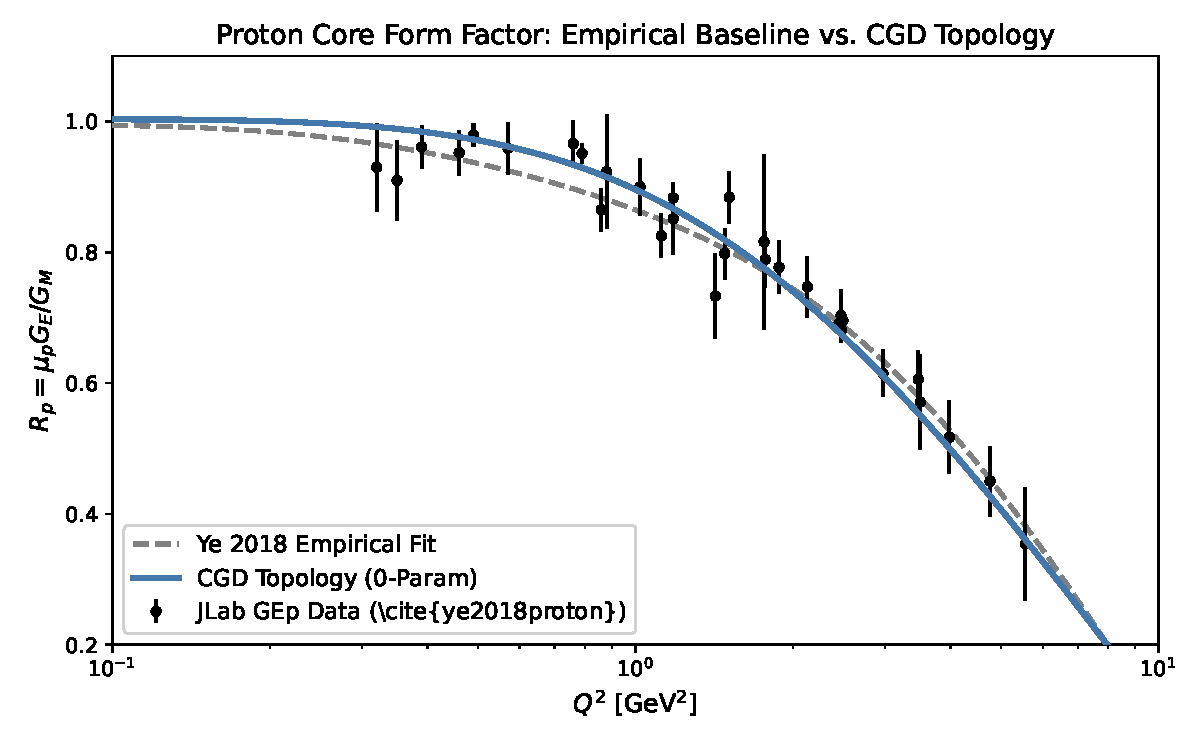
\includegraphics[width=\linewidth]{cgd_appendix_plot.pdf}
    \caption{\todo{Explain the proton radius plot thoroughly}}
    \label{fig:proton_radius}
\end{figure}


\bibliography{refs}

\end{document}
